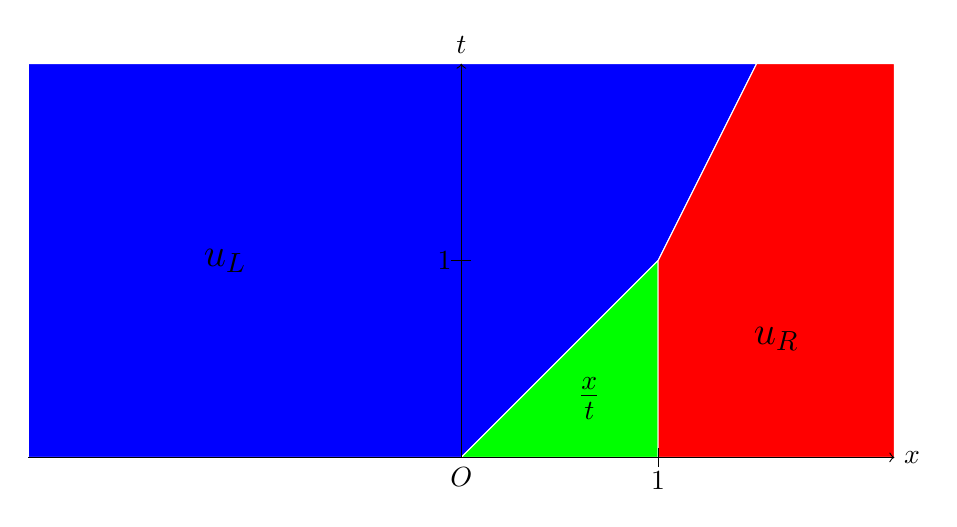
\begin{tikzpicture}[scale=2.5]
\draw[color=white, fill=blue] (-2.2,0) -- (0,0) -- (1,1) -- (1.5,2) -- (-2.2,2) -- cycle;
\draw (-1.2,1) node {\Large{$u_L$}};

\draw[color=white, fill=green] (0,0) -- (1,0) -- (1,1) -- cycle;
\draw (0.65,0.3) node {\Large{$\frac{x}{t}$}};

\draw[color=white, fill=red] (1,0) -- (2.2,0) -- (2.2,2) -- (1.5,2) -- (1,1) -- cycle;
\draw (1.6,0.6) node {\Large{$u_R$}};

\draw[->] (-2.2,0) -- (2.2,0);
\draw (2.2,0) node[right] {$x$};
\draw[->] (0,0) -- (0,2);
\draw (0,2) node[above] {$t$};
\draw (0,0) node[below] {$O$};
\draw (1,-0.05) -- (1,0.05);
\draw (1,-0.025) node[below] {$1$};
\draw (-0.05,1) -- (0.05,1);
\draw (0,1) node[left] {$1$};
\end{tikzpicture}